\chapter{Introducción}

\section{Objetivos del trabajo}

En el presente Trabajo Fin de Máster se analiza la epidemiología de los cánceres de hígado y colon-recto, detectando genes que permiten identificar tumores.

\begin{itemize}
	\item En el capítulo 1, 
	\item En el capítulo 2,
\end{itemize}

\section{Cáncer}

El cáncer es una enfermedad en la que se produce una división incontrolada de las células \cite{AmericanCancerSociety2015}. Aunque generalmente se habla del cáncer como una única enfermedad se trata en realidad de un conjunto de enfermedades, existiendo más de 100 tipos distintos de cáncer \cite{NationalCancerInstitute2015}.\\

El cáncer es una enfermedad genética, esto es, causada por cambios en los genes que controlan las funciones celulares \cite{NationalCancerInstitute2015}. En general, el proceso de creación del cáncer es complejo y multifactorial: a menudo el causante no es un solo elemento, sino la combinación e interacción de distintos factores ambientales y genéticos \cite{Migliore2012}.\\

Los factores causantes del cáncer se pueden clasificar principalmente en tres categorías:
\begin{enumerate}
	\item Factores no modificables. Son elementos que no se pueden cambiar, como la edad o la herencia genética \cite{WorldHealthOrganization2014, WorldHealthOrganization2020}.
	\item Factores modificables o prevenibles, como el tabaco, el alcohol, la dieta o la exposición a distintos carcinógenos \cite{Cogliano2011}.
	\item Otros factores. Algunas circunstancias no se corresponden a ninguna de las categorías anteriores ya que algunos de sus aspectos no se pueden cambiar. Es el caso de  factores socioeconómicos (como cobertura sanitaria en el lugar de residencia o privación económica) y factores reproductivos u hormonales (como toma de anticonceptivos, lactancia materna o terapia hormonal sustitutiva en mujeres menopáusicas) \cite{WorldHealthOrganization2020}.
\end{enumerate}

A continuación se introducen dos tipos de cáncer con los que se trabajará más adelante: el cáncer de hígado y el cáncer de colon-recto.

\subsection{Cáncer de hígado}

\subsubsection{Anatomía y funciones del hígado}

El hígado es el órgano interno más grande y pesado del cuerpo humano, está situado en el cuadrante superior derecho del abdomen, debajo de las costillas, y está compuesto principalmente por dos lóbulos \cite{Abdel-Misih2010}.\\

\textbf{Figura 1}. \textbf{Anatomía del abdomen humano.} Ilustración de Ties van Brussel.
\begin{center}
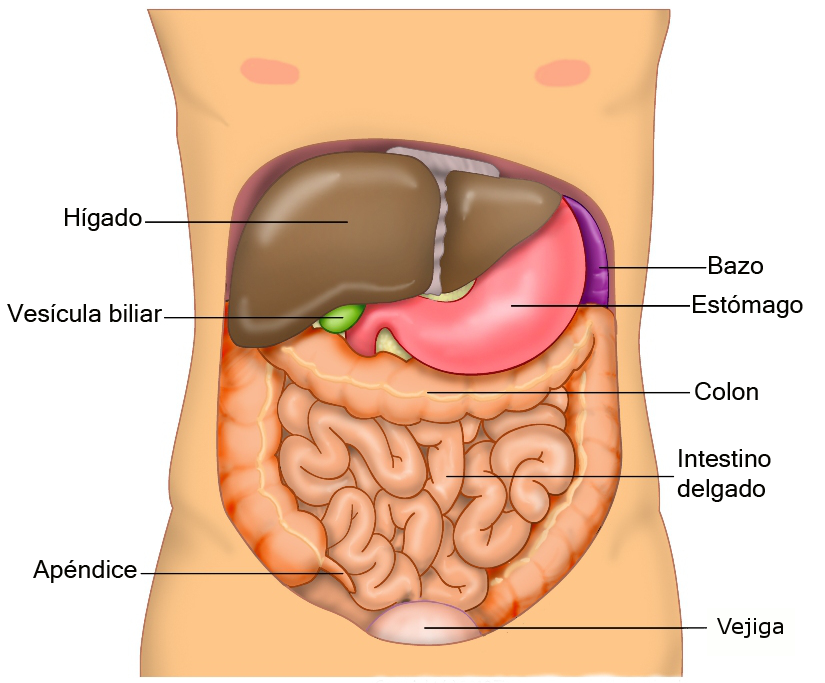
\includegraphics[width=.70\textwidth]{figuras/anatomia_higado.png} \\
\end{center}

Las funciones del hígado son múltiples y diversas. Las principales son procesar, particionar y metabolizar macronutrientes, regular el volumen de sangre, apoyar al sistema inmune, eliminar sustancias químicas como el alcohol y otras drogas y producir bilis para absorber grasas \cite{Trefts2017}. Es un órgano imprescindible para la vida.

\subsubsection{Factores de riesgo}

Uno de los factores de riesgo más comunes del cáncer de hígado es la presencia de cirrosis, o sustitución de células sanas de hígado por tejido cicatrizado. La cirrosis puede producirse por varias causas, siendo las más habituales el consumo excesivo de alcohol y la infección con el virus de la hepatitis B o C \cite{AmericanCancerSociety2019}. Otros factores de riesgo son el tabaco, la obesidad, padecer diabetes tipo II y consumir esteroides anabólicos \cite{AmericanCancerSociety2019, Marrero2005}.\\

La prevención del cáncer de hígado se basa en reducir la exposición a factores de riesgo como el tabaco y el alcohol, y en vacunarse contra la hepatitis B \cite{AmericanCancerSociety2019}.

\subsection{Cáncer de colon-recto}

Los cánceres de colon, recto, unión rectosigmoidea y ano (\textcolor{red}{C18-C21}) a menudo se estudian agrupados por tener características muy similares.

\subsubsection{Anatomía y funciones del colon-recto}

El colon tiene 3 funciones principales: absorción de agua y electrolitos, producción y absorción de vitaminas y movimiento de heces hacia el recto para su eliminación por el ano \cite{Azzouz2020}.\\

\newpage
\textbf{Figura 2}. \textbf{Anatomía del intestino humano.} Ilustración de Ties van Brussel.
\begin{center}
	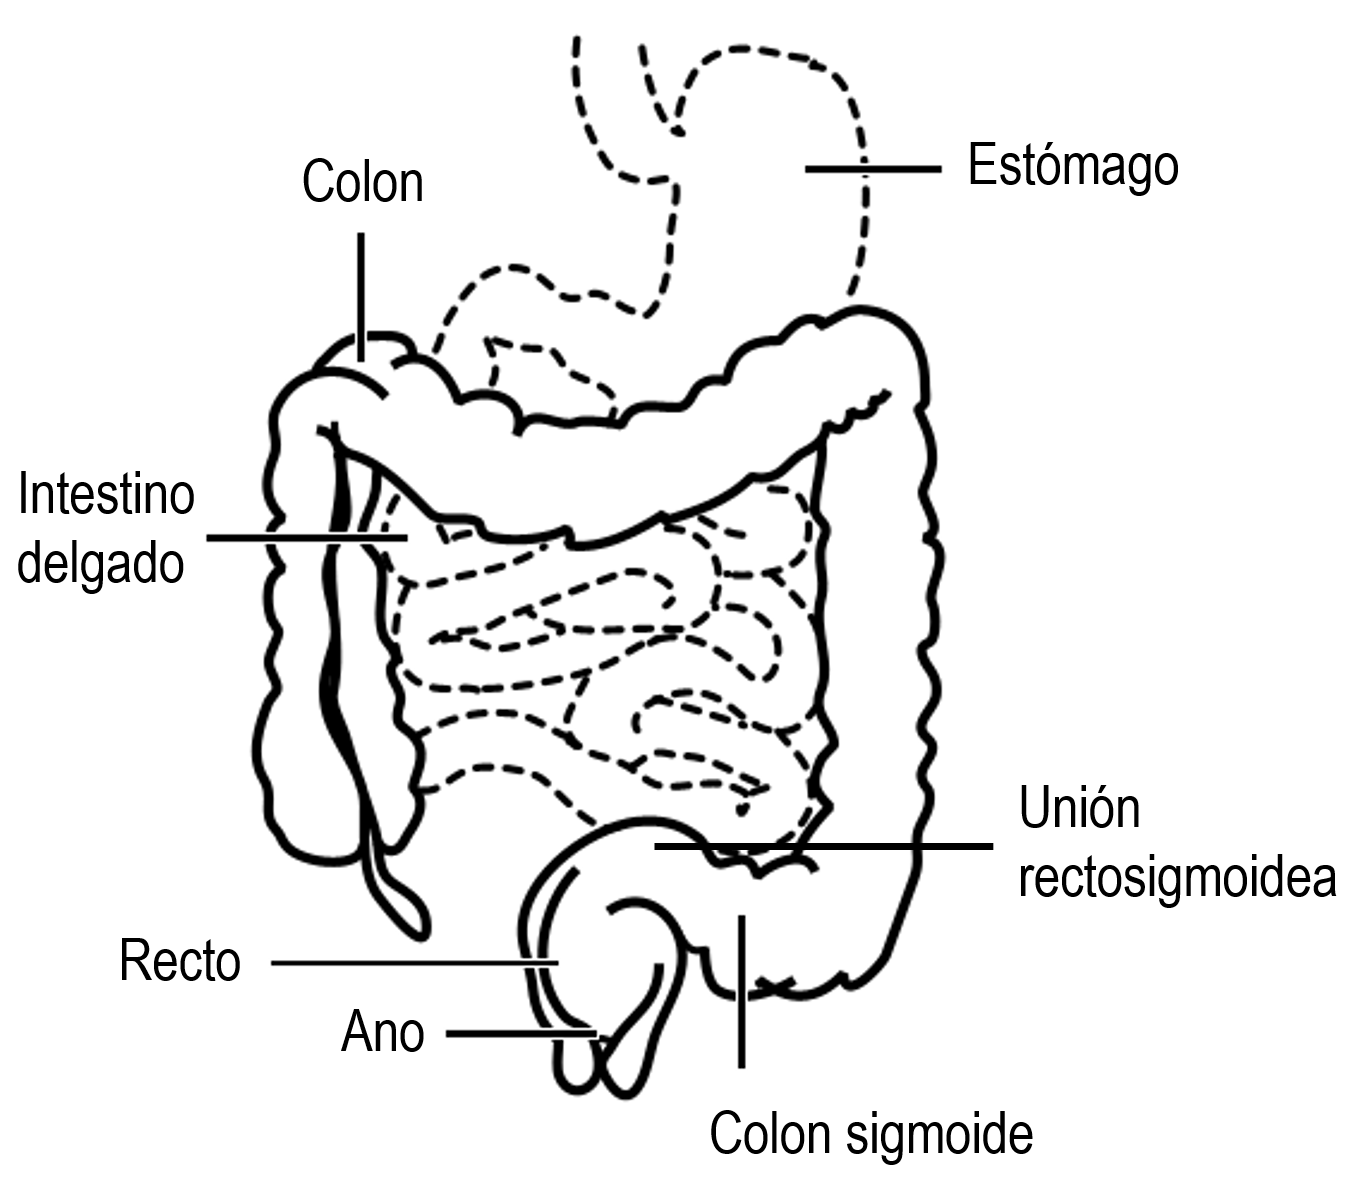
\includegraphics[width=.70\textwidth]{figuras/anatomia_cr.png} \\
\end{center}

\subsubsection{Factores de riesgo}

Entre los factores de riesgo del cáncer de colon-recto se puede distinguir entre factores modificables y no modificables.\\

Entre los factores de riesgo que son modificables destacan el sobrepeso, la inactividad física, las dietas con alto consumo de carnes rojas o procesadas, y el consumo de tabaco y alcohol \cite{AmericanCancerSociety2020}.\\

Una edad superior a 50 años, padecer diabetes tipo 2 y tener antecedentes personales o familiares de cáncer de colon-recto, pólipos o enfermedad intestinal inflamatoria, como colitis ulcerosa y enfermedad de Crohn, son algunos de los factores de riesgo no modificables \cite{AmericanCancerSociety2020}. También existen algunos síndromes hereditarios como el síndrome de Lynch que aumentan las posibilidades de padecer cáncer de colon-recto \cite{Lynch2003}.\\

Para intentar prevenir el cáncer de colon-recto se deben cambiar aquellos factores que son modificables: realizar ejercicio, mantener una dieta saludable y evitar el consumo de tabaco y alcohol. Además, en los últimos años se están implementando programas de cribado de cáncer de colon-recto para detectar pólipos o diagnosticar el cáncer en etapas iniciales mediante análisis como pruebas de sangre oculta en heces o colonoscopias \cite{Levin2008}.\\

\section{Ciencias -ómicas}

\textcolor{red}{Principales con descripción + mencionar otras}

\subsection{Secuenciación del genoma?}

\textcolor{red}{Human Genome Project, ...}

\textcolor{red}{DEGs, }

\subsection{Transcriptómica}

\textcolor{red}{Daniel: La
	genómica estudia el genoma como tal (Cromosomas, mutaciones y
	variaciones tanto de nucleótidos concretos como de regiones del genoma),
	sin embargo la transcriptómica estudia las transcripciones de los genes,
	transcripciones que luego son convertidas a proteínas. Tanto RNA-seq
	como microRNA, se enmarcan en el ámbito de transcriptómica.}


